\documentclass{article}
\usepackage[utf8]{inputenc}
\usepackage{graphicx}
\usepackage{float}
\floatstyle{boxed} 
\restylefloat{figure}
\begin{document}
\title{Exercise 5 of the Computer Vision course at the
  University of Helsinki in May 2018}

\author{\emph{Konsta Kutvonen}}
\maketitle



\newpage
\section{Exercises}
\subsection{Hands-on}
This took about two hours.
\newpage

\begin{verbatim}
import cv2
import numpy as np
from matplotlib import pyplot as plt

frame_idx = 0;

def next_frame_pair():
    global frame_idx
    fl = '{:08d}'.format(frame_idx)
    fr = '{:08d}'.format(frame_idx+1)
    print(fl, fr)
    frame_idx +=2
    return (cv2.imread('frames/'+fl+'.jpeg'),
            cv2.imread('frames/'+fr+'.jpeg'))

stereo = cv2.StereoSGBM_create(numDisparities=16, blockSize=25)

img = None
dx = 0

while True:
    imgLc, imgRc = next_frame_pair()
    imgL = cv2.cvtColor(imgLc, cv2.COLOR_BGR2GRAY)
    imgR = cv2.cvtColor(imgRc, cv2.COLOR_BGR2GRAY)
    #print(imgL, imgR)
    if img is None:
        img = np.zeros((imgL.shape[0],2*imgL.shape[1],3), np.float32)
        dx = imgL.shape[1]

    disparity=stereo.compute(imgL, imgR)
    da = np.array(disparity,dtype=np.float32)
    da /= np.max(da)
    da = np.dstack([da]*3)
    da[disparity<0] = (0,0,255)

    print(np.min(disparity), np.max(disparity))

    img[:imgL.shape[0], :dx] = imgLc.copy()/255.0
    img[:imgL.shape[0], dx:] = da.copy()

    cv2.imshow('disparity', img)
    k = cv2.waitKey(30) & 0xff
    if k == 27:
        break
    elif k == ord('s'):
        cv2.imwrite('stereoD.png',img)

frame_idx = 0;
def next_frame():
    global frame_idx
    f = '{:08d}'.format(frame_idx)
    print(f)
    frame_idx +=2
    return cv2.imread('frames/'+f+'.jpeg')

frame1 = next_frame()
prvs = cv2.cvtColor(frame1,cv2.COLOR_BGR2GRAY)
hsv = np.zeros_like(frame1)
hsv[...,1] = 255
while(1):
    frame2 = next_frame()
    next = cv2.cvtColor(frame2,cv2.COLOR_BGR2GRAY)
    flow = cv2.calcOpticalFlowFarneback(prvs,next, None, 0.5, 3, 15, 3, 5, 1.2, 0)
    mag, ang = cv2.cartToPolar(flow[...,0], flow[...,1])
    hsv[...,0] = ang*180/np.pi/2
    hsv[...,2] = cv2.normalize(mag,None,0,255,cv2.NORM_MINMAX)
    bgr = cv2.cvtColor(hsv,cv2.COLOR_HSV2BGR)
    cv2.imshow('frame2',bgr)
    k = cv2.waitKey(30) & 0xff
    if k == 27:
        break
    elif k == ord('s'):
        cv2.imwrite('opticalfb.png',frame2)
        cv2.imwrite('opticalhsv.png',bgr)
    prvs = next

cv2.destroyAllWindows()

frame_idx = 0;
def next_frame():
    global frame_idx
    f = '{:08d}'.format(frame_idx)
    print(f)
    frame_idx +=2
    return cv2.imread('frames/'+f+'.jpeg')

feature_params = dict( maxCorners = 100,
                       qualityLevel = 0.3,
                       minDistance = 7,
                       blockSize = 7 )
lk_params = dict( winSize  = (15,15),
                  maxLevel = 2,
                  criteria = (cv2.TERM_CRITERIA_EPS | cv2.TERM_CRITERIA_COUNT, 10, 0.03))
color = np.random.randint(0,255,(100,3))
old_frame = next_frame()
old_gray = cv2.cvtColor(old_frame, cv2.COLOR_BGR2GRAY)
p0 = []
while(1):
    if len(p0)==0:
        p0 = cv2.goodFeaturesToTrack(old_gray, mask = None, **feature_params)
        mask = np.zeros_like(old_frame)
    frame = next_frame()
    frame_gray = cv2.cvtColor(frame, cv2.COLOR_BGR2GRAY)
    p1, st, err = cv2.calcOpticalFlowPyrLK(old_gray, frame_gray, p0, None, **lk_params)
    if not p1 is None:
        good_new = p1[st==1]
        good_old = p0[st==1]
        for i,(new,old) in enumerate(zip(good_new,good_old)):
            a,b = new.ravel()
            c,d = old.ravel()
            mask = cv2.line(mask, (a,b),(c,d), color[i].tolist(), 2)
            frame = cv2.circle(frame,(a,b),5,color[i].tolist(),-1)
            img = cv2.add(frame,mask)
            cv2.imshow('frame',img)
        k = cv2.waitKey(30) & 0xff
        if k == 27:
            break
        old_gray = frame_gray.copy()
        if k == 27:
            break
        elif k == ord('s'):
            cv2.imwrite('lkflow.png',frame)
            cv2.imwrite('lkflowmod.png',img)
        p0 = good_new.reshape(-1,1,2)
cv2.destroyAllWindows()
cap.release()
\end{verbatim}
\newpage
\begin{figure}
\center
            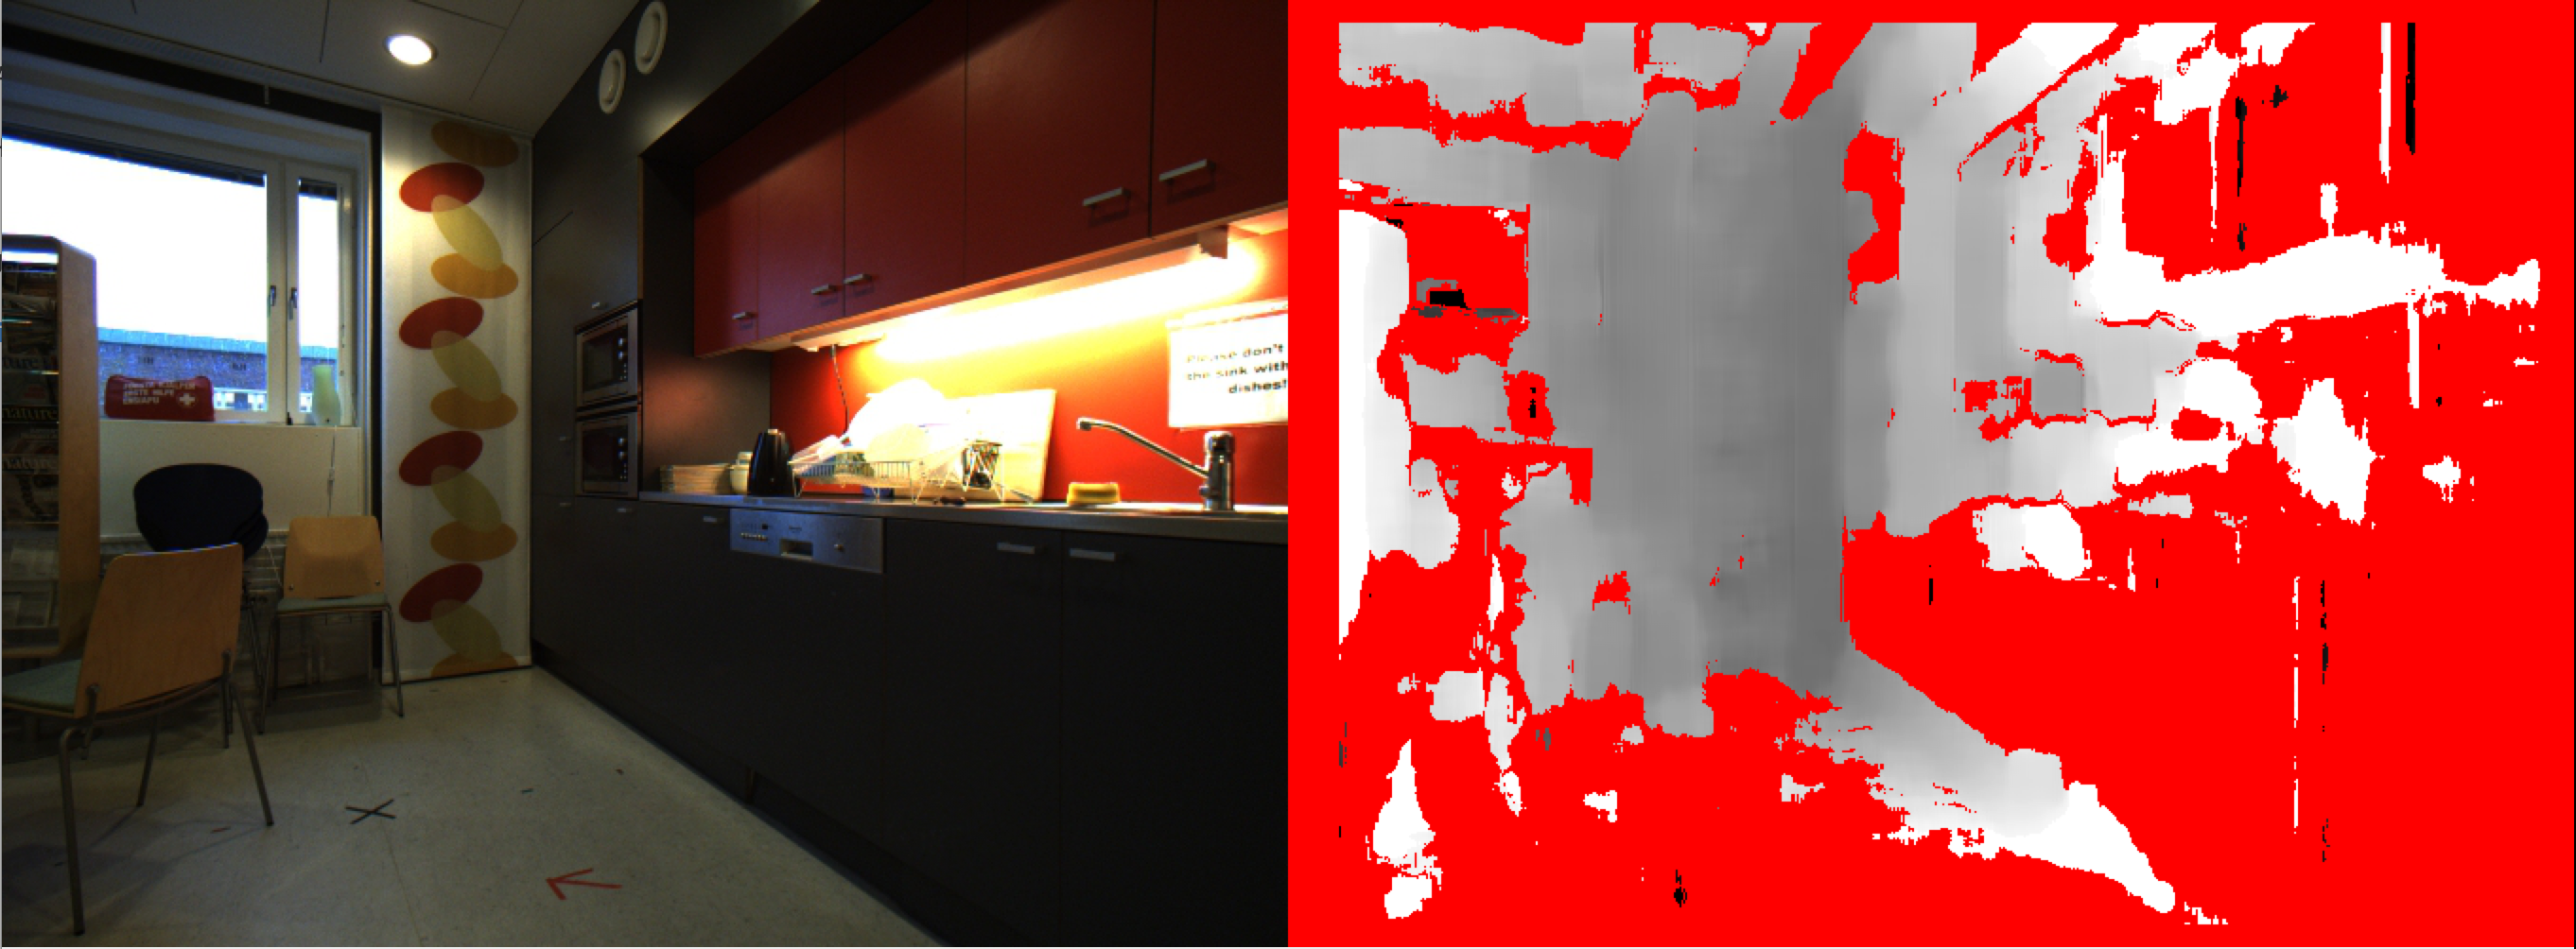
\includegraphics[width=1\textwidth]{stereo}
\caption{StereoBM original and disparity}
\end{figure}       
\begin{figure}
\center
            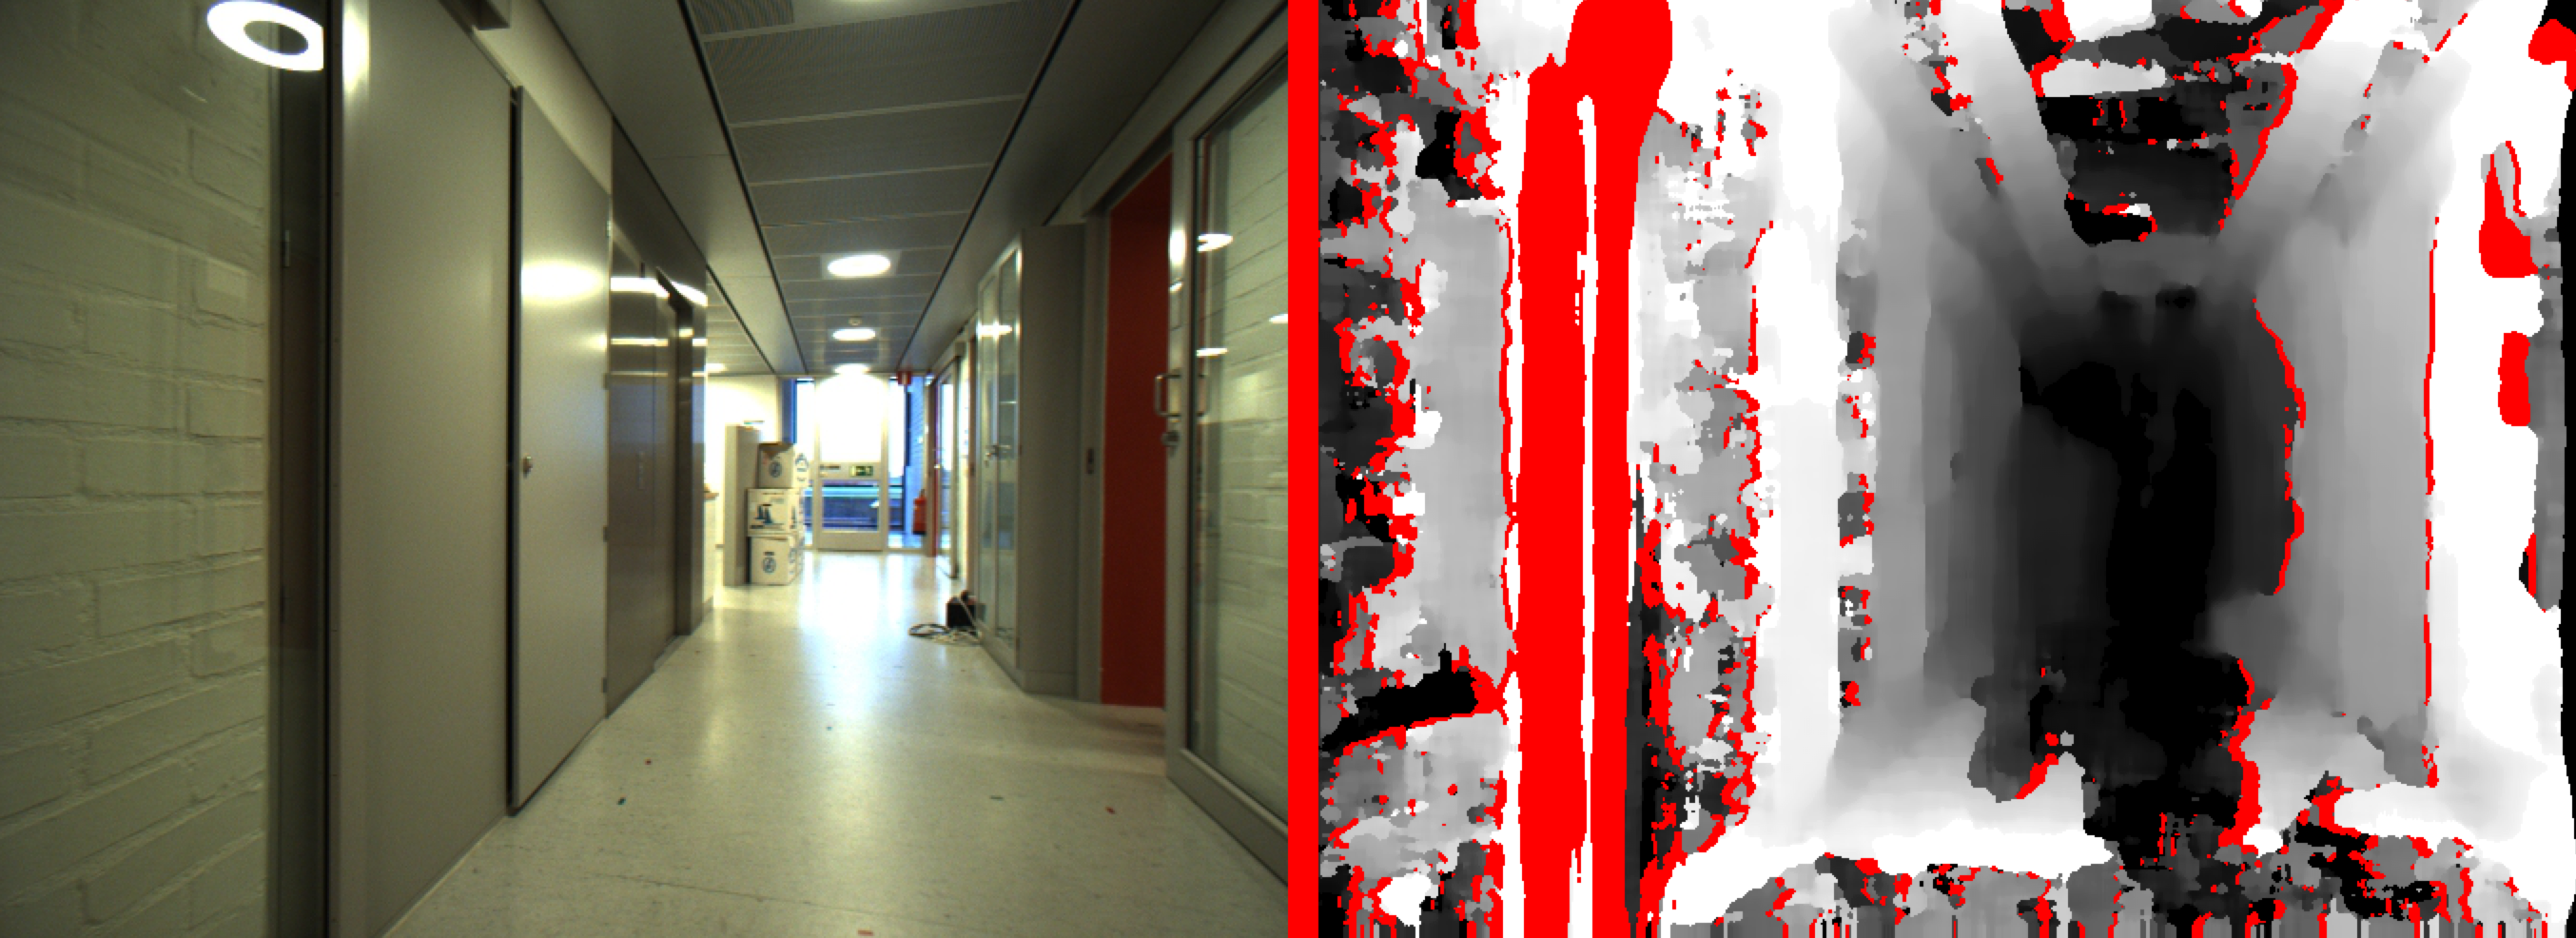
\includegraphics[width=1\textwidth]{stereosgbm}
\caption{StereoSGBM original and disparity}
\end{figure}       
\begin{figure}
\center
            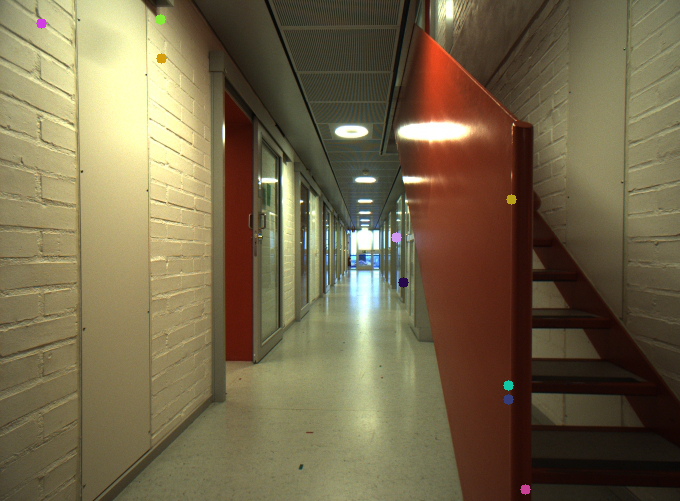
\includegraphics[width=1\textwidth]{lkflow}
            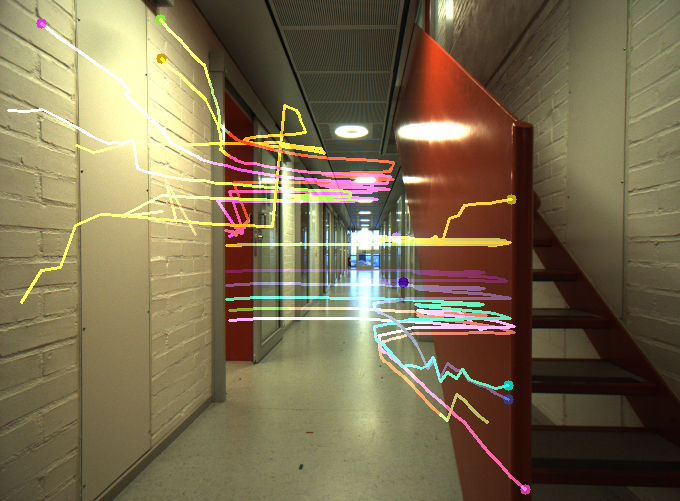
\includegraphics[width=1\textwidth]{lkflowmod}
\caption{Lukas Canade flow fields with calcOpticalFlowPyrLK()}
\end{figure}       
\begin{figure}
\center
            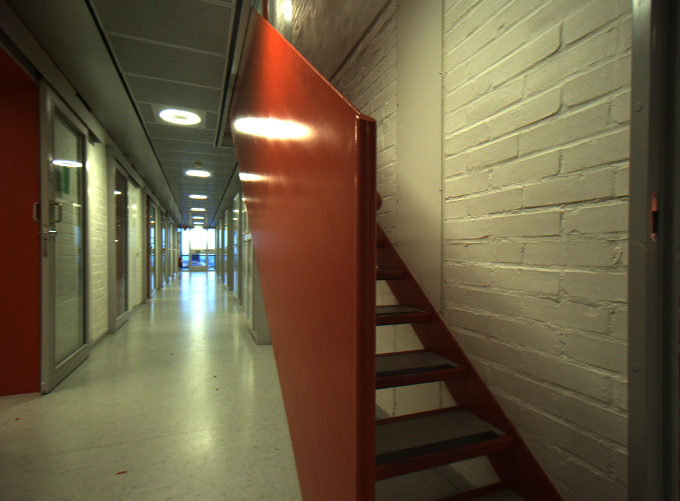
\includegraphics[width=1\textwidth]{opticalfb}
            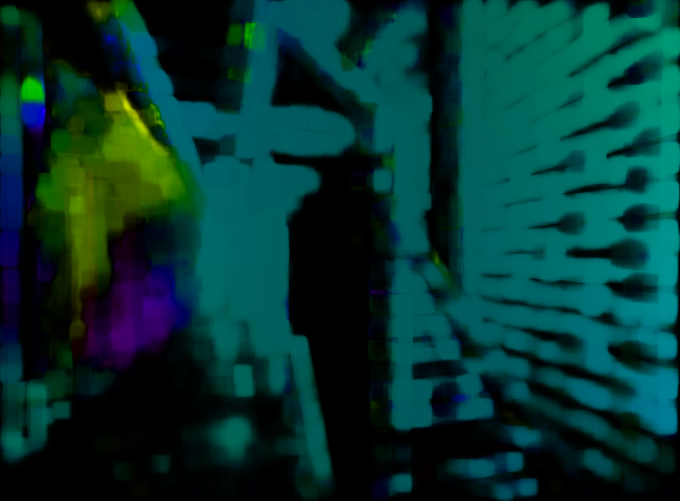
\includegraphics[width=1\textwidth]{opticalhsv}
\caption{Optical flow with calcOpticalFlowFarneback() }
\end{figure}       
\newpage
\end{document}
